\section{Auswertung}
\label{sec:Auswertung}

\subsection{Wheatstonesche Brücke} \label{sec:wheatausw}

Die Werte der bei der Messung bekannten Widerstände sind in \autoref{tab:wheatbekannt} aufgetragen.
\begin{table}
  \centering
  \caption{Werte der bekannten Widerstände.}
  \label{tab:wheatbekannt}
  \begin{tabular}{lcc}
    \toprule
     & Messung 1 & Messung 2  \\
    \midrule
    \multicolumn{3}{c}{ Bestimmung von $R_{\text{x, 13}}$ } \\
    $R_2 \mathbin{/} \unit{\ohm}$ & 1000 & 500 \\
    $R_3 \mathbin{/} \unit{\ohm}$ &  240 & 388 \\
    $R_4 \mathbin{/} \unit{\ohm}$ &  760 & 612 \\
    \midrule 
    \multicolumn{3}{c}{ Bestimmung von $R_{\text{x. 18}}$ } \\
    $R_2 \mathbin{/} \unit{\ohm}$ & 1000 & 500 \\
    $R_3 \mathbin{/} \unit{\ohm}$ &  190 & 321 \\
    $R_4 \mathbin{/} \unit{\ohm}$ &  810 & 679 \\
    \bottomrule
  \end{tabular}
\end{table}

Die baubedingte Abweichung für $R_2$ beträgt $\qty{0.2}{\percent}$. 
Die Abweichung für das Verhältnis $\frac{R_3}{R_4}$ beträgt $\qty{0.5}{\percent}$.
Mit den bekannten Werten $R_2$, $R_3$ und $R_4$ und der (\ref{eq:Rx}) ergibt sich
mithilfe der Fehlerrechnung nach \autoref{sec:Fehlerrechnung} für die gemittelten unbekannten Widerstände
\begin{align*}
  \bar{R}_\text{x, 13} &= \qty{316.4(1.2)}{\ohm} \quad \text{und} \\
  \bar{R}_\text{x, 18} &= \qty{235.5(9)}{\ohm} \, .
\end{align*}


\subsection{Kapazitätsmessbrücke} \label{sec:kapazausw}

Die Werte der bekannten Kenngrößen sind in \autoref{tab:kapazbekannt} zu sehen.
\begin{table}
  \centering
  \caption{Werte der bekannten Kapazitäten und Widerstände.}
  \label{tab:kapazbekannt}
  \begin{tabular}{cc}
    \toprule
     & Messung 1  \\
    \midrule
    \multicolumn{2}{c}{ Bestimmung von $C_{\text{x, 8}}$ und $R_{\text{x, 8}}$ } \\
    $C_2 \mathbin{/} \unit{\nano\farad}$     & 450 \\
    $R_2 \mathbin{/} \unit{\ohm}$            & 500 \\
    $R_3 \mathbin{/} \unit{\ohm}$            & 388 \\
    $R_4 \mathbin{/} \unit{\ohm}$            & 612 \\
    \bottomrule
  \end{tabular}
\end{table}

Die Abweichung für $C_2$ beträgt $\qty{0.2}{\percent}$, wobei die Abweichung des Potentiometers beibleibt
und die Abweichung für $R_2$ ist nun $\qty{3}{\percent}$. 
Die Berechnung von $C_\text{c}$ und $R_\text{c}$ geschieht nach (\ref{eq:Rx}):
\begin{align*}
  C_\text{x, 8} &= \qty{233.7(1.3)}{\nano\farad} \, , \\
  R_\text{x, 8} &= \qty{433.0(13.0)}{\ohm} \, .
\end{align*}


\subsection{Induktivitätsmessbrücke} \label{sec:induktausw}

Die Werte der bekannten Kenngrößen sind in \autoref{tab:unduktbekannt} zu sehen.
\begin{table}
  \centering
  \caption{Werte der bekannten Induktivität und der Widerstände.}
  \label{tab:unduktbekannt}
  \begin{tabular}{lccc}
    \toprule
     & Messung 1 & Messung 2 & Messung 3  \\
    \midrule
    \multicolumn{4}{c}{ Bestimmung von $L_{\text{x, 17}}$ und $R_{\text{x, 17}}$ } \\
    $L_2 \mathbin{/} \unit{\milli\henry}$ &  14,6 &  27,5 &  20,1\\
    $R_2 \mathbin{/} \unit{\ohm}$         &  30,0 &  33,0 &  42,0\\
    $R_3 \mathbin{/} \unit{\ohm}$         & 745,0 & 606,0 & 678,0\\
    $R_4 \mathbin{/} \unit{\ohm}$         & 255,0 & 396,0 & 322,0\\
    \bottomrule
  \end{tabular}
\end{table}

Die baubedingten Abweichungen sind dieselben wie im vorangegangenem \autoref{sec:kapazausw}.
Die Abweichung für die Induktivität $L_2$ der Spule beträgt $\qty{0.2}{\percent}$.
Die gemittelten Werte für $L_\text{x, 17}$ und $R_\text{x, 17}$ ergeben sich nach (\ref{eq:L_x}) und (\ref{eq:induktR_x}) zu
\begin{align*}
  \bar{L}_\text{x, 17} &= \qty{42.4(1)}{\milli\henry} \quad \text{und} \\
  \bar{R}_\text{x, 17} &= \qty{75.5(1.4)}{\ohm} \, .
\end{align*}

\subsection{Maxwell Brücke} \label{sec:maxwausw}

Die Werte der bekannten Kenngrößen sind in \autoref{tab:maxwbekannt} ersichtlich.
\begin{table}
  \centering
  \caption{Werte der bekannten Kapazität und der Widerstände.}
  \label{tab:maxwbekannt}
  \begin{tabular}{lcc}
    \toprule
     & Messung 1 & Messung 2  \\
    \midrule
    \multicolumn{3}{c}{ Bestimmung von $L_{\text{x, 17}}$ und $R_{\text{x, 17}}$ } \\
    $C_4 \mathbin{/} \unit{\nano\farad}$  &  450 &  660 \\
    $R_2 \mathbin{/} \unit{\ohm}$         & 1000 & 1000 \\
    $R_3 \mathbin{/} \unit{\ohm}$         &   85 &   60 \\
    $R_4 \mathbin{/} \unit{\ohm}$         &  960 &  700 \\
    \bottomrule
  \end{tabular}
\end{table}

Die Abweichungen der beiden einstellbaren Widerstände $R_3$ und $R_4$ betragen jeweils  $\qty{3}{\percent}$.
Die des Widerständs $R_2$ und der Kapazität $c_4$ des Kondensators betragen beide $\qty{0.2}{\percent}$.
Die gemittelten Werte für $L_\text{x, 17}$ und $R_\text{x, 17}$ ergeben sich nach (\ref{eq:maxwL_x}) und (\ref{eq:Rx}) zu
\begin{align*}
  \bar{L}_\text{x, 17} &= \qty{47.2(1.4)}{\milli\henry} \quad \text{und} \\
  \bar{R}_\text{x, 17} &= \qty{105.0(4.0)}{\ohm} \, .
\end{align*}


\subsection{Wien-Robinson-Messbrücke} \label{sec:wienausw}

In dieser Messreihe wird die Frequenzabhängigkeit einer Wien-Robinson-Messbrücke untersucht.
Hierzu wird das Verhältnis der Brückenspannung $U_\text{Br}$ zur Speisespannung $U_\text{S}$
gegen $\Omega = \frac{\nu}{\nu_0}$ abgetragen. Wobei sich die Frequenz $\nu_0$, 
bei der die Brückenspannung verschwinden sollte, sich ergibt durch:
\begin{align*}
  \omega_{0} &=\frac{1}{R C}=\frac{1}{\qty{1}{\kilo\ohm} \cdot \qty{660}{nF}}= \qty{1515.15}{Hz} \\
  \Leftrightarrow \nu_{0} &=\frac{\omega_{0}}{2 \pi} = \qty{241.14}{Hz} \, .
\end{align*}
Das Minimum wird, im Vergleich dazu sehr genau, bei $\nu_\text{0, exp} = \qty{241}{Hz}$ gemessen.

\begin{table} [h]
  \centering
  \caption{Gemessene Spannungen in Abhängigkeit von der Frequenz am Sinusspannungsgenerator.}
  \label{tab:spannung}
  \begin{tabular}{c c}
    \toprule
    $\nu \mathbin{/} \mathrm{Hz}$ &  $U_\text{Br} \mathbin{/} \mathrm{mV}$ \\
    \midrule
        20 &     280 \\
        40 &     260 \\
        80 &     200 \\
       160 &      80 \\
       230 &      32 \\
       232 &      26 \\
       234 &      20 \\
       236 &      15 \\
       238 &      10 \\
       240 &       4 \\
       241 &       2 \\
       242 &       5 \\
       244 &      10 \\
       246 &      15 \\
       248 &      20 \\
       250 &      26 \\
       320 &      55 \\
       640 &     180 \\
      1280 &     245 \\
      2560 &     280 \\
      5020 &    1000 \\
     10040 &    1400 \\
     20080 &    1000 \\
     30000 &     750 \\
    \bottomrule
    \end{tabular}
\end{table}

Die dabei gemessene Speisespannung erweist sich zu jeder Frequenz als konstant: $U_\text{S} = \qty{4}{V}$.
In \autoref{fig:plot} sind die Messdaten und die Theoriekurve nach (\ref{eq:Wien2}) dargestellt.
\begin{figure}[H]
  \centering
  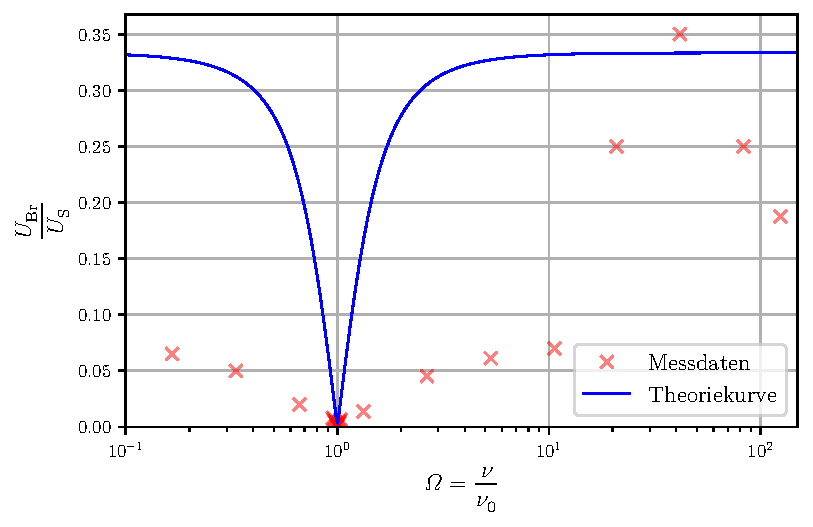
\includegraphics[width=\textwidth]{plot.pdf}
  \caption{Vergleich von Messdaten mit der Theoriekurve.}
  \label{fig:plot}
\end{figure}